\section{Introducción}

\subsection{Qué es question answering}

\begin{frame}
  \frametitle{¿Qué es question answering?}
  \begin{block}{Question Answering}<3->
      Es el proceso automatizado de generación de respuestas concretas para preguntas formuladas en lenguaje natural.
  \end{block}
  \bigskip

 \begin{alertblock}{Question}<2->
      ¿Quién desarrolló la teoría de la relatividad?
  \end{alertblock}

  \begin{columns}<3->
      \begin{column}{.5\textwidth}
      \end{column}
      \begin{column}{.1\textwidth}
      \begin{tikzpicture}[>=stealth, rotate border/.style={shape border uses incircle, shape border rotate=270}]
              \node[rotate border=-40, fill=black, minimum height=1.5cm, single arrow, single arrow head extend=.3cm, single arrow head indent=.1cm, inner sep=1.5pt] (arrow) {};
          \end{tikzpicture}
      \end{column}
      \begin{column}{.3\textwidth}
          %Question Answering
      \end{column}
      \begin{column}{.5\textwidth}

      \end{column}
  \end{columns}

  \begin{exampleblock}{Answer}<2->
      Albert Einstein.
  \end{exampleblock}
\end{frame}

\begin{frame}
\frametitle{Ejemplo IR}
\begin{figure}
  \centering
    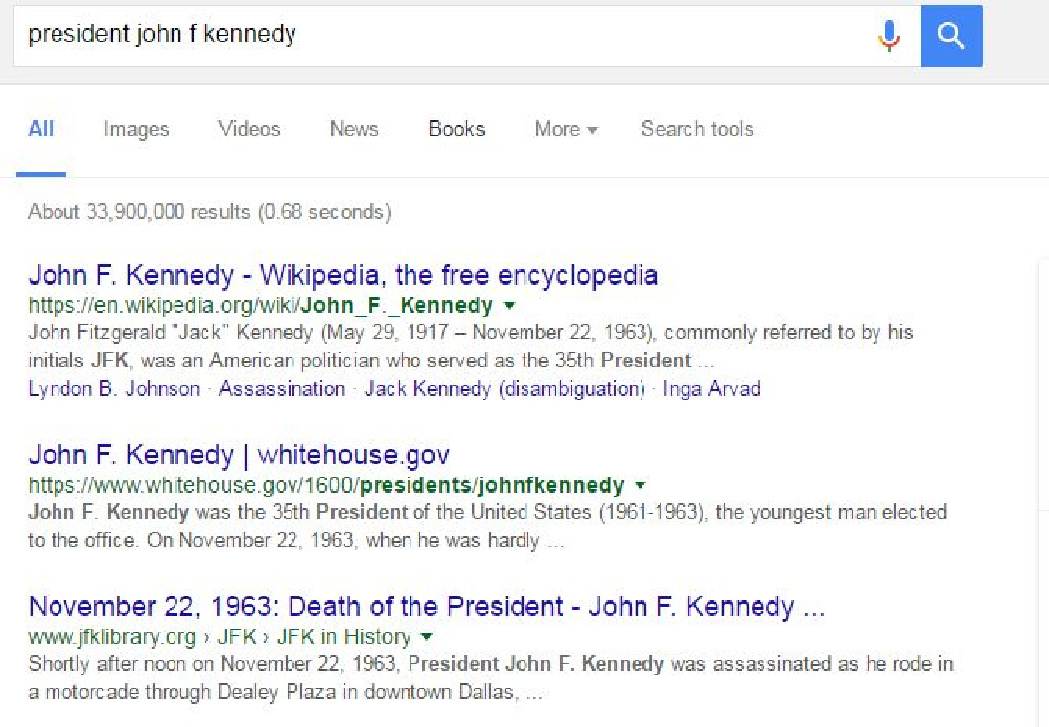
\includegraphics[scale=.35]{graficos/i-r-example}
  \caption{Google como sistema de Information Retrieval}
  \label{fig:qa-example}
\end{figure}
\end{frame}


\begin{frame}
\frametitle{Ejemplo QA}
\begin{figure}
  \centering
    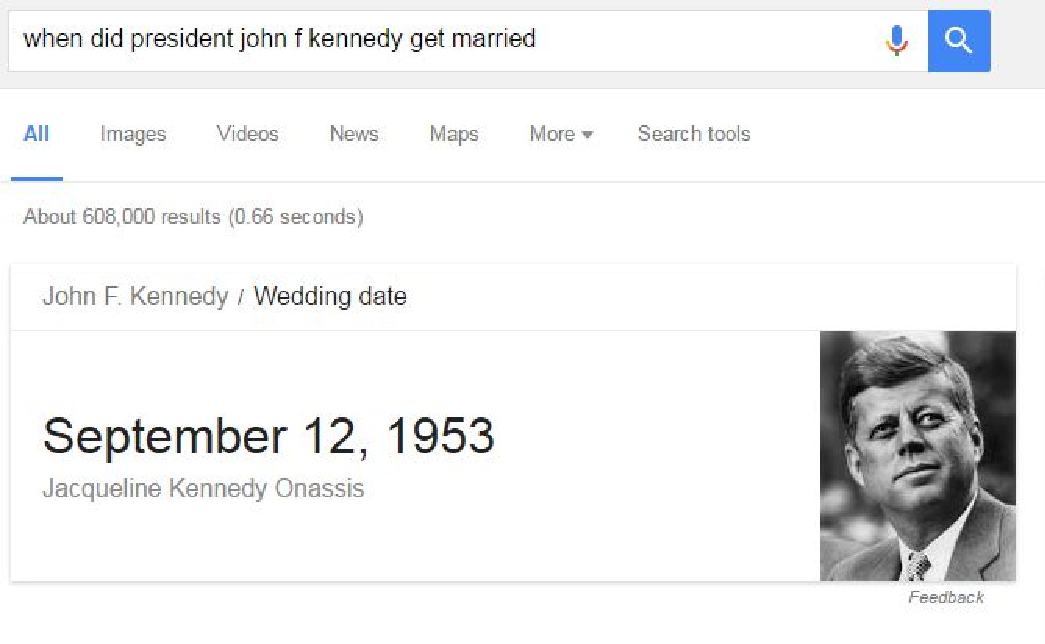
\includegraphics[scale=.5]{graficos/q-a-example}
  \caption{Google como sistema de Question Answering}
  \label{fig:qa-example}
\end{figure}
\end{frame}


\begin{frame}
  \frametitle{Clasificación}
  \begin{block}{Generalidad del dominio}<2->
    \begin{itemize}
      \item Dominio abierto o dominio cerrado
    \end{itemize}
  \end{block}
  \begin{block}{Tipo de datos}<3->
    \begin{itemize}
      \item Estructurados (Bases de datos)
      \item No estructurados (Colecciones de textos)
    \end{itemize}
  \end{block}
  \begin{block}{Soporte de preguntas}<4->
    \begin{itemize}
      \item Fácticas, listas, definiciones, modo, razón
      \item Cláusulas de tiempo, sin respuesta, etc.
    \end{itemize}
  \end{block}
\end{frame}


\subsection{Qué es esta tesis}

\begin{frame}
  \frametitle{Qué es esta tesis}
    \begin{block}{Brevemente}<2->
      Implementamos dos sistemas de question answering más o menos decentes.
    \end{block}
    \begin{exampleblock}{Dominio cerrado con soporte para inglés / Popescu World}<3->
      \begin{itemize}
          \item Base de datos relacional de juguete
          \item Modelo teórico de \textit{tratabilidad semántica}
          \item Traduce preguntas a consultas SQL
      \end{itemize}
    \end{exampleblock}
    \begin{alertblock}{Dominio abierto con soporte multilingüe / Multilingual Qanus}<4->
      \begin{itemize}
          \item Wikipedia(s) como base de conocimientos
          \item Framework Qanus y librería Freeling
          \item Basado en IR + NLP + heurísticas
      \end{itemize}
    \end{alertblock}
\end{frame}